%%% kontraktionsmodus 2, 1st order, stufe 10 ist wichtig.
\begin{tikzpicture}
\begin{axis}[height=0.35\textheight,width=0.45\textwidth,style={font=\footnotesize},grid=major,grid style={dotted},align=center,xlabel={Tensorstufe},ylabel={Durchsatz [GFlops]},title={Kontraktionsmodus 2},xtick={2,3,4,5,6,7,8,9,10},xticklabels={2,3,4,5,6,7,8,9,10},ybar,bar width=4.5pt]
\addplot
coordinates{(2.000,17.544)+-(0.201,0.201) (3.000,9.230)+-(1.161,1.161) (4.000,15.792)+-(1.615,1.615) (5.000,25.482)+-(0.868,0.868) (6.000,34.267)+-(0.436,0.436) (7.000,33.761)+-(0.450,0.450) (8.000,32.969)+-(0.402,0.402) (9.000,34.257)+-(0.271,0.271) (10.000,34.664)+-(0.328,0.328) };\label{coord_perf_float:2_2}
\addplot
coordinates{(2.000,16.748)+-(0.196,0.196) (3.000,10.971)+-(1.212,1.212) (4.000,15.539)+-(1.033,1.033) (5.000,24.166)+-(0.578,0.578) (6.000,31.744)+-(0.325,0.325) (7.000,30.820)+-(1.390,1.390) (8.000,30.771)+-(0.498,0.498) (9.000,31.394)+-(0.218,0.218) (10.000,32.110)+-(0.264,0.264) };\label{coord_perf_float:4_2}
\end{axis}
\end{tikzpicture}
%\footnotesize Dargestellt sind über die Tensorgröße gemittelten \textbf{Durchsätze in Gflops} der \textbf{Tensor}"=\textbf{Vektor}"=\textbf{Multiplikation}. \textbf{TLib-SB-PB1} \ref{coord_perf_float:1_1},\textbf{TLib-SB-PB3} \ref{coord_perf_float:2_1},\textbf{TLib-LB-PB1} \ref{coord_perf_float:3_1},\textbf{TLib-LB-PB2} \ref{coord_perf_float:4_1}. Daten sind in \textbf{Floating-Point<Single>} codiert.

%%% kontraktionsmodus 1, 2st order, stufe 10 ist wichtig.
\begin{tikzpicture}
\begin{axis}[height=0.35\textheight,width=0.45\textwidth,style={font=\footnotesize},grid=major,grid style={dotted},align=center,xlabel={Tensorstufe},ylabel={Laufzeit [ms]},title={Kontraktionsmodus 1},xtick={2,3,4,5,6,7,8,9,10},xticklabels={2,3,4,5,6,7,8,9,10},ybar,bar width=4.5pt]
\addplot
coordinates{(2.000,33.094)+-(18.625,18.625) (3.000,58.138)+-(31.058,31.058) (4.000,37.753)+-(19.881,19.881) (5.000,22.722)+-(12.468,12.468) (6.000,16.154)+-(8.982,8.982) (7.000,16.461)+-(9.272,9.272) (8.000,16.720)+-(9.275,9.275) (9.000,16.168)+-(8.961,8.961) (10.000,15.919)+-(8.835,8.835) };\label{coord_time_float:2_1}
\addplot
coordinates{(2.000,33.770)+-(19.059,19.059) (3.000,53.029)+-(29.197,29.197) (4.000,35.008)+-(18.219,18.219) (5.000,22.725)+-(12.525,12.525) (6.000,17.269)+-(9.632,9.632) (7.000,17.840)+-(9.952,9.952) (8.000,17.964)+-(10.047,10.047) (9.000,17.047)+-(9.393,9.393) (10.000,17.161)+-(9.497,9.497) };\label{coord_time_float:4_1}
\end{axis}
\end{tikzpicture}